\documentclass[11pt,twoside]{article}

\usepackage{amsmath}
\usepackage{amssymb}
\usepackage{amsthm}
\usepackage{courier} % Required for the courier font
\usepackage{extramarks} % Required for headers and footers
\usepackage{fancyhdr} % Required for custom headers
\usepackage{graphicx} % Required to insert images
\usepackage{lastpage} % Required to determine the last page for the footer
\usepackage{listings} % Required for insertion of code
\usepackage{lipsum} % Used for inserting dummy 'Lorem ipsum' text into the template
\usepackage{mathtools}
\usepackage{subcaption}

\usepackage[margin=1in]{geometry}
\usepackage[usenames,dvipsnames]{color} % Required for custom colors

\begin{document}

\title{CSC411 - Project \#2}
\author{Michael Wong - [Student Number]\\Yijin (Catherine) Wang - 998350476}
\maketitle

\clearpage

\section*{Part 1}
\paragraph{Question}
Describe the dataset of digits. In your report, include 10 images of each of the digits. You may find matplotlib’s subplot useful.

\paragraph{Answer}
Please see the images of each digits below. For the same digit, some images have thicker lines (like ``8'' in the second column) and some have thiner lines (like ``8" in the third column). Some digit images are straight (like ``1" in the first column) and some digits are rotated (like ``1" in the ninth column). Most digits are clear to be identified manually but some digits are not clear (like the ``6" in the seventh column). 

\begin{figure*}[h]
	\centering
	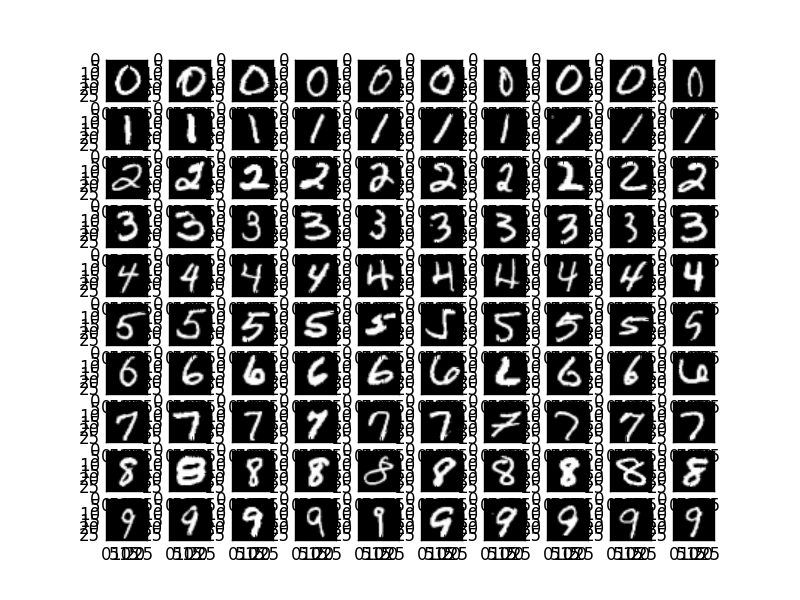
\includegraphics[scale=0.8]{part1.png}
	\caption*{10 images of digits from 0 to 9}
\end{figure*}

\clearpage

\section*{Part 2}

\paragraph{Question}
Implement a function that computes the network below.
\begin{figure*}[h]
	\centering
	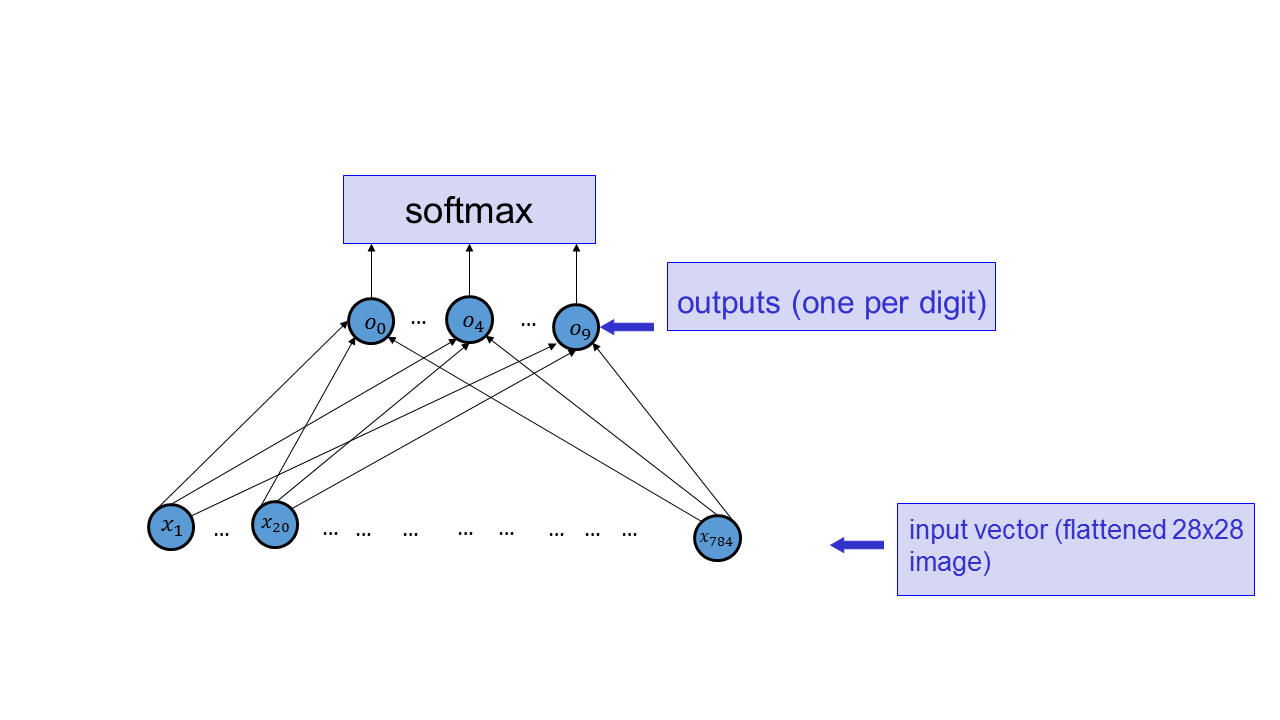
\includegraphics[scale=0.5]{logreg.png}
\end{figure*}
The $o$'s here should simply be linear combinations of the $x$'s (that is, the activation function in the output layer is the identity). Supecifically, use $o_i = \sum_{j}w_{ji}x_j+b_i$. Include the listing of your implementation in your report for this Part.

\paragraph{Answer}
Please see the source code of the function below:

\begin{lstlisting}[language=Python]
def softmax(y):
    '''Return the output of the softmax function for the matrix of output y. y
    is an NxM matrix where N is the number of outputs for a single case, and M
    is the number of cases'''
    return exp(y)/tile(sum(exp(y),0), (len(y),1))


def lin_combin(w, b, x):
    o = (dot(w.T, x) + b)
    return softmax(o)
\end{lstlisting}


\clearpage

\section*{Part 3}
We would like to use the sum of the negative log-probabilities of all the training cases as the cost function.

\subsection*{Part 3(a)}
\paragraph{Question}
Compute the gradient of the cost function with respect to the weight $w_{ij}$. Justify every step. You may refer to Slide 7 of the One-Hot Encoding lecture , but note that you need to justify every step there, and that your cost function is the sum over all the training examples.

\paragraph{Answer}
We could calculate $\frac{\partial p_j}{\partial o_i}$ in two cases:
\begin{enumerate}
\item If $j = i$,
\begin{align*}
\frac{\partial p_i}{\partial o_i} &= \frac{e^{o_i}}{\sum_{k}e^{o_k}} - \frac{e^{o_i}}{\sum_{k}e^{o_k}} \cdot \frac{e^{o_i}}{\sum_{k}e^{o_k}}\\
&= p_i(1 - p_i)
\end{align*}
\item If $j \neq i$,
\begin{align*}
\frac{\partial p_j}{\partial o_i} &= -\frac{e^{o_j}}{\sum_{k}e^{o_k}} \cdot \frac{e^{o_i}}{\sum_{k}e^{o_k}}\\
&= -p_jp_i
\end{align*}
\end{enumerate}
In summary,
\begin{equation}
    \frac{\partial p_j}{\partial o_i} =
    \begin{cases*}
      p_i(1 - p_i) &, if $j = i$ \\
      -p_jp_i &, if $j \neq i$
    \end{cases*}
\end{equation}
\[\frac{\partial C}{\partial p_j} = -\frac{y_j}{p_j}\]
\begin{align*}
\frac{\partial C}{\partial o_{i}} &= \sum_{j}\frac{\partial C}{\partial p_j} \frac{\partial p_j}{\partial o_i}\\
&= \sum_{j, j \neq i}\frac{\partial C}{\partial p_j} \frac{\partial p_j}{\partial o_i} + \frac{\partial C}{\partial p_i} \frac{\partial p_i}{\partial o_i}\\
&= \sum_{j, j \neq i}(-\frac{y_j}{p_j}) \cdot (-p_jp_i) - \frac{y_i}{p_i} \cdot p_i(1 - p_i)\\
&= \sum_{j, j \neq i}y_jp_i - y_i + yip_i\\
&= \sum_{j}y_jp_i - y_i\\
\end{align*}
Because $\sum_{j}y_j = 1$, $\sum_{j}y_jp_i = p_i$. Then,
\begin{align*}
\frac{\partial C}{\partial o_{i}} &= p_i - y_i
\end{align*}
For the following equation, let $j$ refers to the input size (number of $x$ per sample) and $i$ refers to the output size (number of $o$ per sample), and $k$ refers to the training set size (number of samples).\\
\\
$X$ is the input matrix with dimension $n \times m$, where $n$ is the number $x$ (related to $j$) and $m$ is the sample size (related to $k$). $P$ is the calculated result matrix after using softmax with dimension $d \times m$, where $d$ is the output size (number of outputs per sample, related to $i$). $Y$ is the expected output with the same dimension as $P$.
\[\frac{\partial C}{\partial o_{ik}} = p_{ik} - y_{ik}\]
\[\frac{\partial o_{ik}}{\partial w_{ij}} = x_{jk}\]
\begin{align*}
\frac{\partial C}{\partial w_{ij}} &= \sum_{k}\frac{\partial C}{\partial o_{ik}} \cdot \frac{\partial o_{ik}}{\partial w_{ij}}\\
&= \sum_{k}x_{jk}(p_{ik} - y_{ik})\\
&= X(P - Y)^T
\end{align*}
\subsection*{Part 3(b)}
\paragraph{Question}
Write vectorized code that computes the gradient with respect to the cost function. Check that the gradient was computed correctly by approximating the gradient at several coordinates using finite differences. Include the code for computing the gradient in vectorized form in your report.

\paragraph{Answer}
\begin{lstlisting}[language=Python]
def part3b(M):
    """Test gradient for part 3b."""
    
    x1 = M["train8"][0]
    x2 = M["train8"][1]
    x = vstack((x1, x2)).T
    y = array([[1, 0, 0, 0, 0, 0, 0, 0, 0, 0], [1, 0, 0, 0, 0, 0, 0, 0, 0, 0]]).T
    w = zeros((x.shape[0], 10))
    b = zeros((10, 2))
    test_gradient(x, y, b, w)


def test_gradient(x, y, b, w):
    """
    Compare the result of my gradient function NLL_gradient and the gradient get 
    from finite differences method. Test three times on different w_ij.
    """
    
    j_list = [5, 8, 8]
    i_list = [300, 601, 600]
    
    h = 10e-5
    
    for k in range(0, 3):
        i = i_list[k]
        j = j_list[k]
        g_finite = finite_diff_gradient(x, y, w, b, i, j, h)
        g_mine = NLL_gradient(x, y, w, b)[i, j]
        diff = abs(g_mine - g_finite)
        print("Test "+str(k)+":")
        print("gradient_finite_differences = "+str(g_finite))
        print("gradient_my_function = "+str(g_mine))
        print("difference = "+str(diff))
        print("-------------------------------")    


def finite_diff_gradient(x, y, w, b, i, j, h):
    """
    Use finite difference to calculate the gradient on w_ij with h.
    x: input
    y: expected output
    w: weight
    b: bias
    """
    
    c = NLL(x, y, w, b) 
    new_w = w
    new_w[i, j] += h
    new_c = NLL(x, y, new_w, b) 
    return (new_c - c)/h


def NLL(x, y, w, b):
    p = lin_combin(w, b, x)
    return -sum(y*log(p)) 
    
    
def NLL_gradient(x, y, w, b):
    p = lin_combin(w, b, x)
    return dot(x, (p - y).T)
\end{lstlisting}

\end{document}